\subsection{Results and Discussion}\label{Section:Face-Recognition:Results}

While there \it{should} be 6 different experiments to cover (combinations of 3 different architectures and 2 different training techniques), we accidentally skipped the combination of \it{InceptionNetV3 and triplet loss training} and didn't notice until the very end.
As such, that experiment will not be covered. 
Otherwise, we will try to go through each experiment systematically.
Overall, every experiment achieved fairly decent results.

\begin{enumerate}[left=0pt]
\item \it{NN1 and Triplet Loss Training}

At first glance, the clusters in \Cref{Figure:Face-Recognition:Results:nn1-and-triplet-loss-tsne-sequence} show that the data is fairly clustered with only a couple stray image embeddings.
However, since t-SNE is a probabilistic technique, we must use the other two tools to verify our claim.
In particular, we focus on the distances for \Eunbi in both the boxplot (\Cref{Figure:Face-Recognition:Results:nn1-and-triplet-loss-boxplot}) and medoid table (\Cref{Table:Face-Recognition:Results:nn1-and-triplet-loss-medoid}).
The maximum dispersion the her image embeddings have a distance of 1.2 while the medoid distances can be as low as 1.06 (\Chaeyeon) and 0.79 (\Minju).
This indicates that there can be overlaps between the clusters of these three members (or at the very least, pairwise overlaps).
We make one of two conclusions here (both could occur together):
\begin{enumerate}
    \item We ended training too early.
    This is quite possible as we didn't have an accuracy metric to work with for triplet loss (More on this in \Cref{Section:Face-Recognition:Remarks})
    
    \item The network was not complex enough to learn differentiating features between the members. (Part of the reason we're trying out different architectures!)
\end{enumerate}

\begin{figure}[htbp]
    \centering
    \begin{subfigure}{0.24\textwidth}
        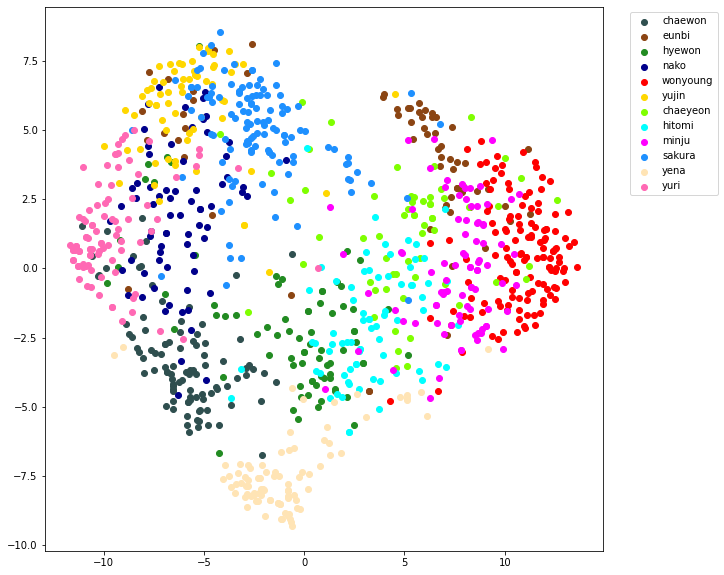
\includegraphics[trim=45 20 100 0, clip, width=\textwidth]{images/faceReco/nn1-and-triplet/tsne-1.png}     
    \end{subfigure}
    \hfill
    \begin{subfigure}{0.24\textwidth}
        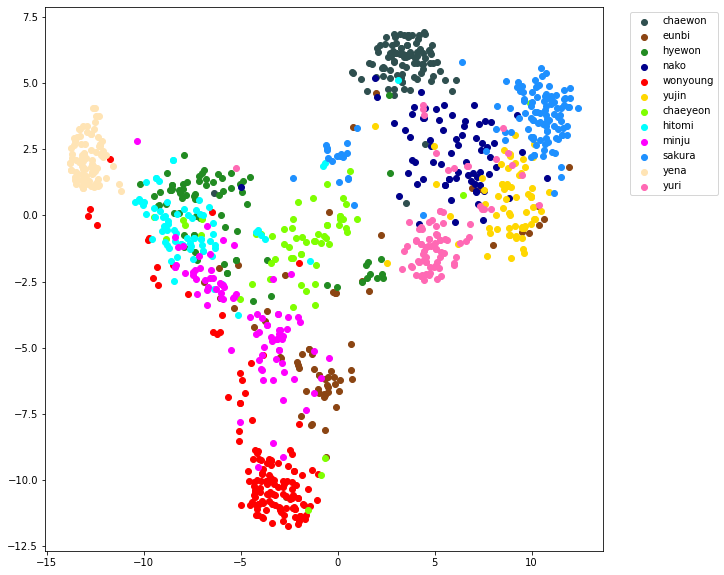
\includegraphics[trim=45 20 100 0, clip, width=\textwidth]{images/faceReco/nn1-and-triplet/tsne-2.png}     
    \end{subfigure}
    \hfill
    \begin{subfigure}{0.24\textwidth}
        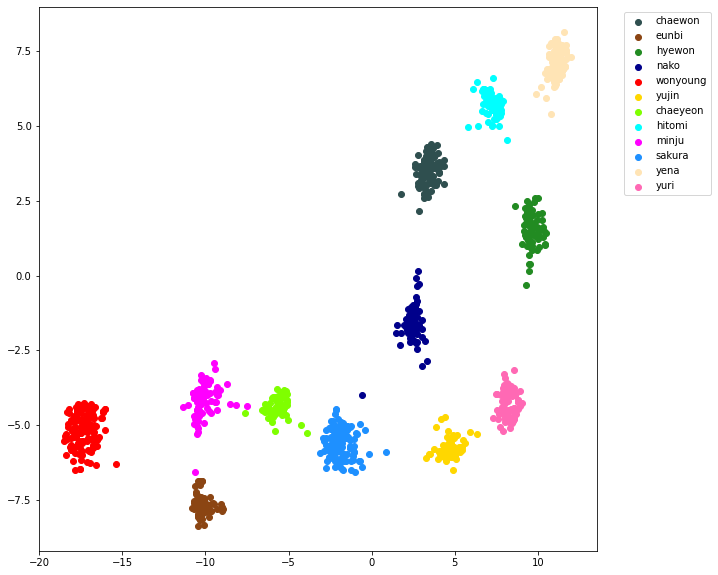
\includegraphics[trim=35 20 100 0, clip, width=\textwidth]{images/faceReco/nn1-and-triplet/tsne-3.png}     
    \end{subfigure}
    \hfill
    \begin{subfigure}{0.24\textwidth}
        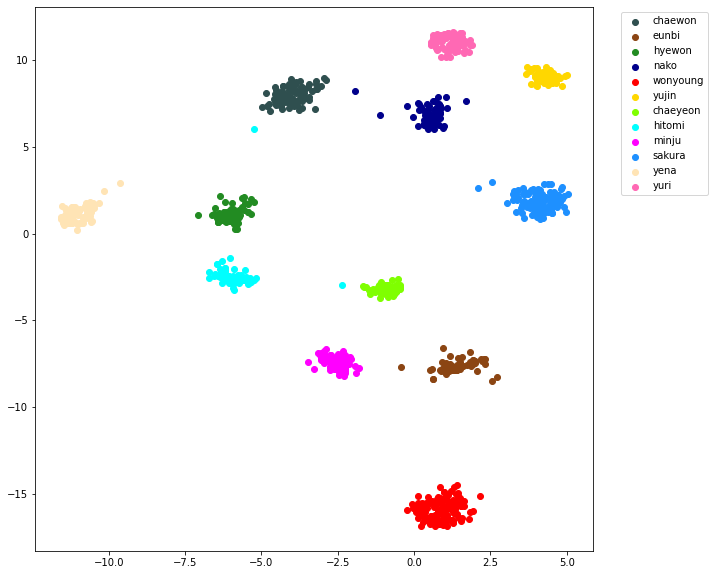
\includegraphics[trim=32 22 100 0, clip, width=\textwidth]{images/faceReco/nn1-and-triplet/tsne-4.png}     
    \end{subfigure}

    \caption{Sequence of t-SNE plots taken at various points during the training of NN1 with the triplet loss technique. From left to right, the plots were taken after training on: 8000 triplets, 16000 triplets, 27520 triplets and 29760 triplets}
    \label{Figure:Face-Recognition:Results:nn1-and-triplet-loss-tsne-sequence}
\end{figure}

\begin{figure}[htbp]
    \centering
    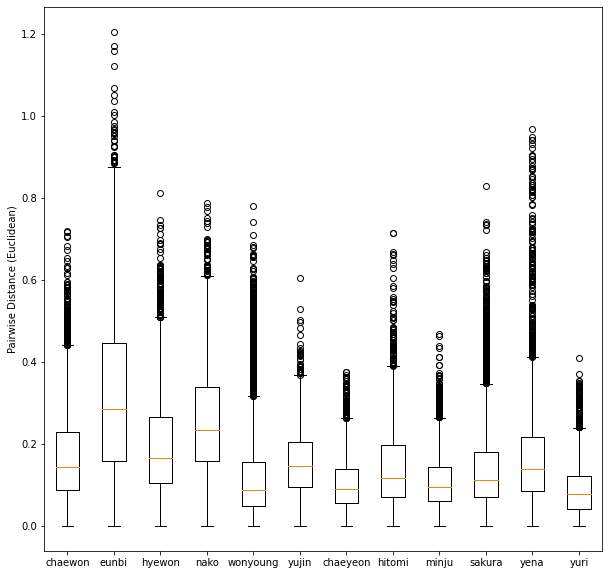
\includegraphics[width=0.7\textwidth]{images/faceReco/nn1-and-triplet/boxplot}
    \caption{Boxplot of pairwise distances for the training of NN1 with the triplet loss technique}
    \label{Figure:Face-Recognition:Results:nn1-and-triplet-loss-boxplot}
\end{figure}

\item \it{NN1 and Binary Classification Training}

The results from this experiment were quite interesting!
First, we note that the cluster sizes are quite small in the expanded image of \Cref{Figure:Face-Recognition:Results:nn1-and-binary-tsne-sequence}.
While t-SNE doesn't play well with true cluster sizing, we can confirm (with \Cref{Figure:Face-Recognition:Results:nn1-and-binary-boxplot}) that, indeed, the dispersion within clusters is quite low.
This is exactly the short whiskers and few outliers we were looking for.

However, on the left hand side of the expanded image, there are two clusters that are overlapping.
We can confirm with \Cref{Table:Face-Recognition:Results:nn1-and-binary-medoid} that \Chaewon\ and \Yena\ have a distance of 0 between their medoids!
Further, we note that the pairwise distance between the image embeddings for \Yena\ and \Chaewon\ (minus a couple outliers) are all 0.
This indicates that our network has learned to send all images of \Yena\ and \Chaewon\ to the same vector\footnote{Insert \it{yet another} JoYuriz joke here} in $\R^{128}$.

Continuing with the analysis of \Cref{Table:Face-Recognition:Results:nn1-and-binary-medoid}, \it{many} of the distances are exactly 2.0.
Since our image embeddings are normalized, this means that our network has learned to send images of each member to their own corner in an $128$-simplex.
This seems almost too good to be true, and truth be told, this interesting behaviour more likely suggests that something went wrong while training.
However, since our implementation of this particular technique worked well with other architectures, we didn't ponder over this too much.
Another equally likely possibility is that we completely overfit for our training data.

\begin{figure}[htbp]
    \centering

    % First Row 
    \begin{subfigure}{0.325\textwidth}
        \centering
        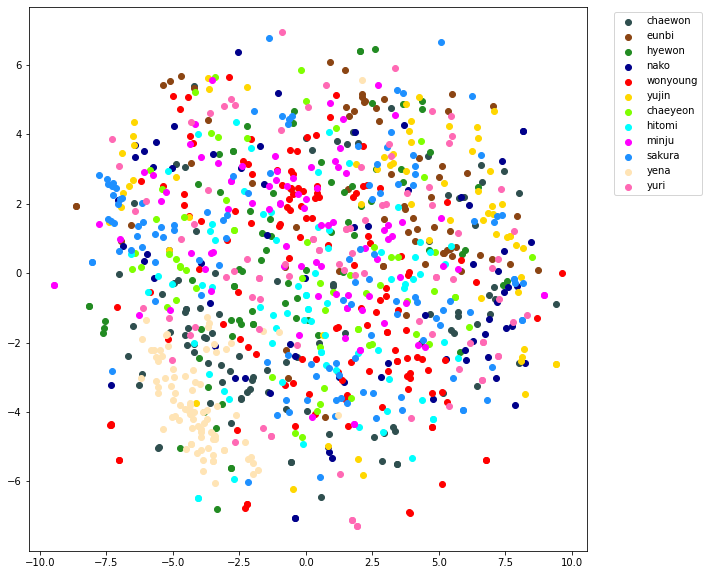
\includegraphics[trim=25 20 100 0, clip, width=\textwidth]{images/faceReco/nn1-and-binary/tsne-1.png}     
    \end{subfigure}
    \hfill
    \begin{subfigure}{0.325\textwidth}
        \centering
        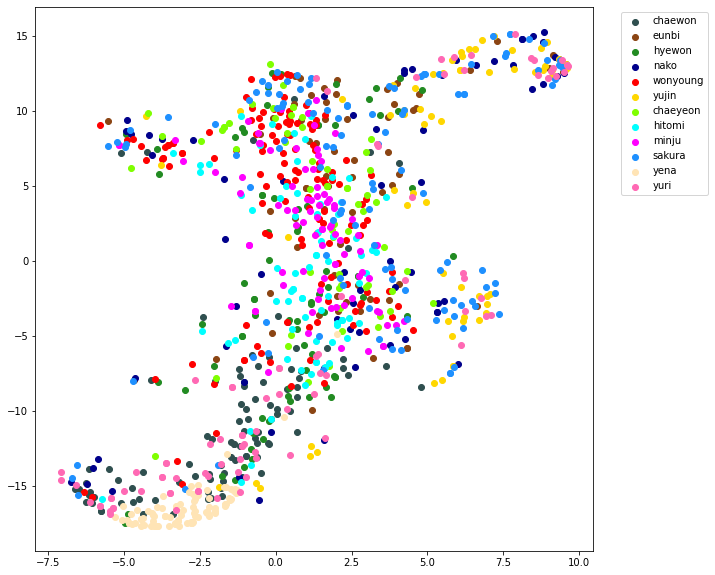
\includegraphics[trim=30 20 100 0, clip, width=\textwidth]{images/faceReco/nn1-and-binary/tsne-2.png}     
    \end{subfigure}
    \hfill
    \begin{subfigure}{0.325\textwidth}
        \centering
        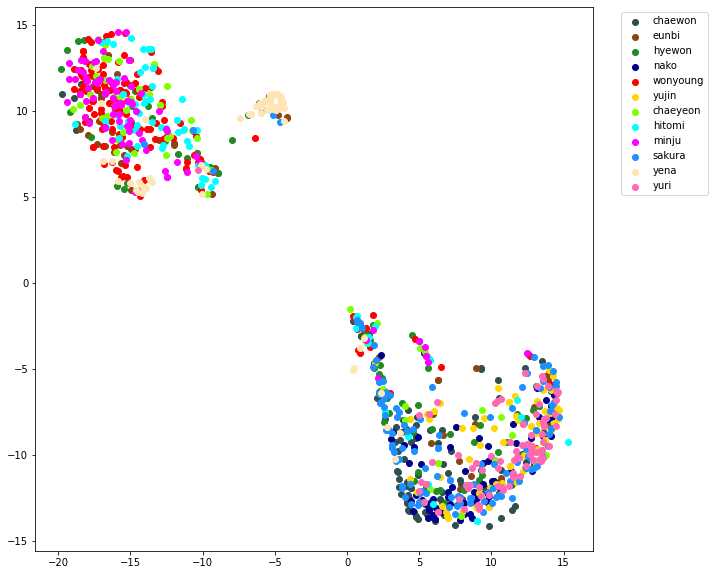
\includegraphics[trim=30 20 100 0, clip, width=\textwidth]{images/faceReco/nn1-and-binary/tsne-3.png}     
    \end{subfigure}

    % Second Row
    \vspace{2mm}
    \begin{subfigure}{0.325\textwidth}
        \centering
        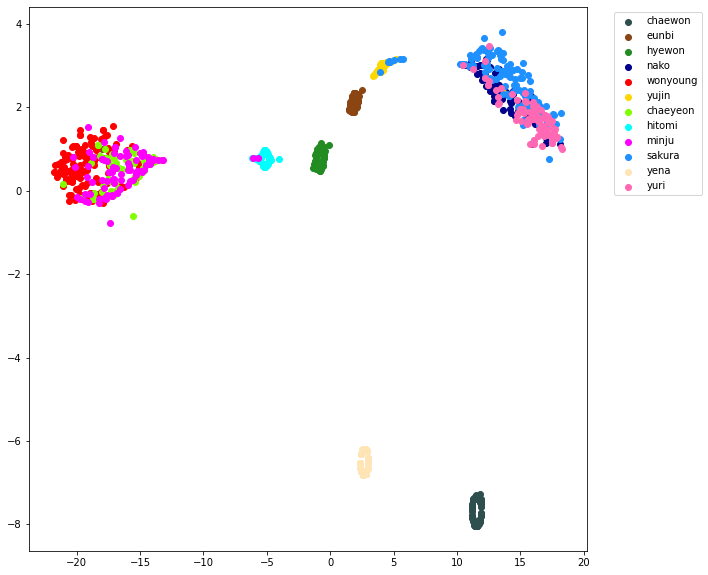
\includegraphics[trim=25 22 100 0, clip, width=\textwidth]{images/faceReco/nn1-and-binary/tsne-4.png}     
    \end{subfigure}
    \hfill
    \begin{subfigure}{0.325\textwidth}
        \centering
        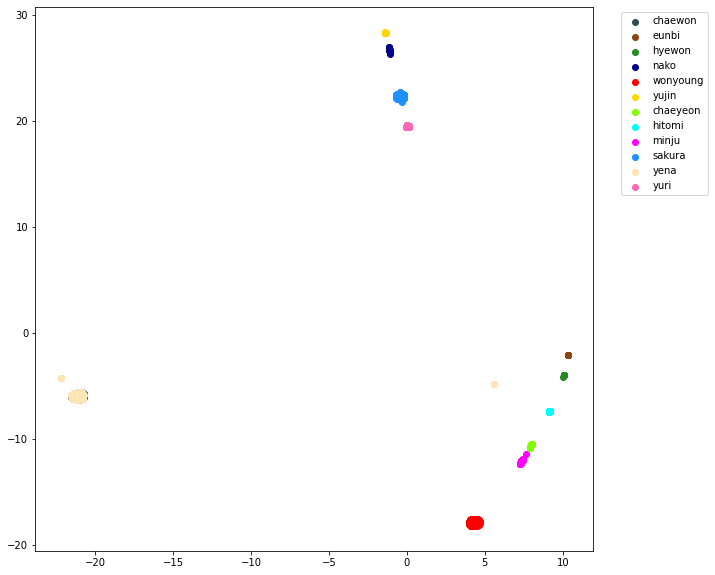
\includegraphics[trim=30 22 100 0, clip, width=\textwidth]{images/faceReco/nn1-and-binary/tsne-5.png}     
    \end{subfigure}
    \hfill
    \begin{subfigure}{0.325\textwidth}
        \centering
        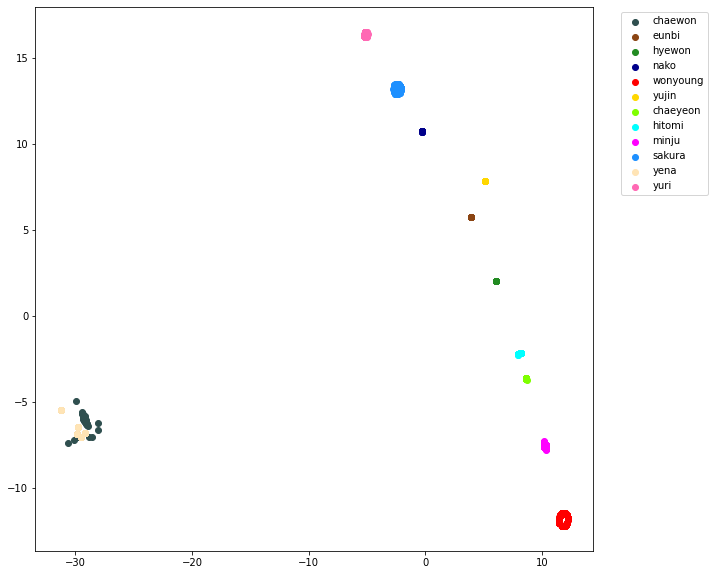
\includegraphics[trim=30 22 100 0, clip, width=\textwidth]{images/faceReco/nn1-and-binary/tsne-6.png}     
    \end{subfigure}

    % Solo
    \vspace{2mm}
    \begin{subfigure}{\textwidth}
        \centering
        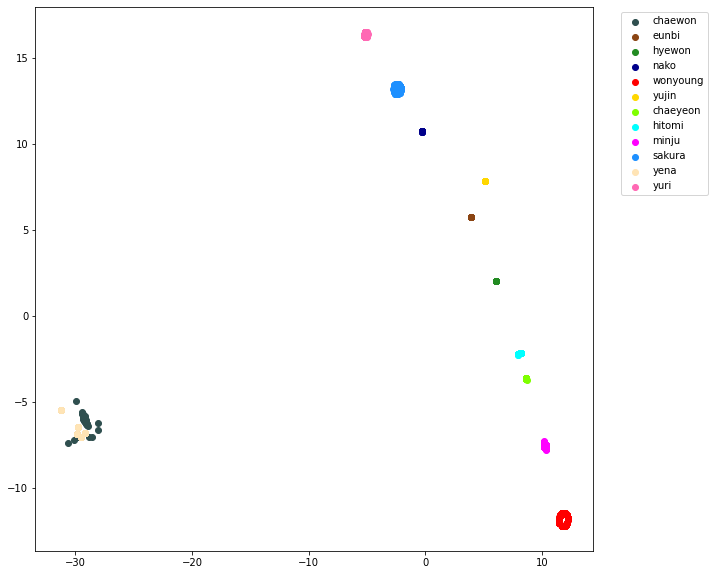
\includegraphics[trim=34 22 100 0, clip, width=0.6\textwidth]{images/faceReco/nn1-and-binary/tsne-6.png}     
    \end{subfigure}

    \caption{
        Sequence of t-SNE plots taken at various points during the training of NN1 with the binary classification technique.
        From left-to-right and top-to-bottom, the plots were taken after training on: 0 (Pre-training plot), 500, 1000, 5000, 10000, and 366000 samples.
        The solo, larger plot is an expanded version of the plot taken at 366000 samples
    }
    \label{Figure:Face-Recognition:Results:nn1-and-binary-tsne-sequence}
\end{figure}

\begin{figure}[htbp]
    \centering
    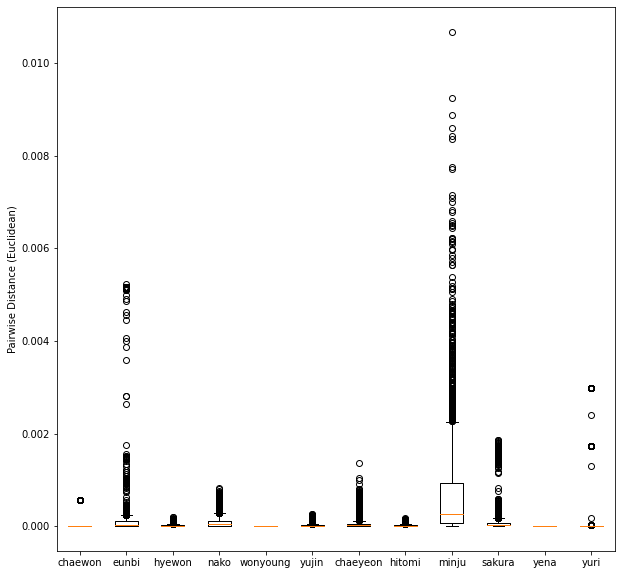
\includegraphics[width=0.7\textwidth]{images/faceReco/nn1-and-binary/boxplot}
    \caption{Boxplot of pairwise distances for the training of NN1 with the binary classification technique}
    \label{Figure:Face-Recognition:Results:nn1-and-binary-boxplot}
\end{figure}


\item \it{NN2 and Triplet Loss}

Recall that NN2 is a much deeper network \cite[Table 2]{facenet}, hence we should expect somewhat better results with NN2 than either of our previous experiments.
We start by looking at the t-SNE plots (\Cref{Figure:Face-Recognition:Results:nn2-and-triplet-tsne-sequence}).
As with our previous experiments, we see what looks to be well-clustered embeddings.
\Cref{Figure:Face-Recognition:Results:nn2-and-triplet-boxplot} tells us that we have intra-cluster distances of up to (around) 0.9 while \Cref{Table:Face-Recognition:Results:nn2-and-triplet-medoid} admits inter-cluster distances $>1$ for the most part.
As such, the three tools tell us that this experiment was fairly successful!
The network has learned to minimized distances within clusters and pushed entire clusters far away from each other.

\begin{figure}[htbp]
    \centering
    \begin{subfigure}{0.325\textwidth}
        \centering
        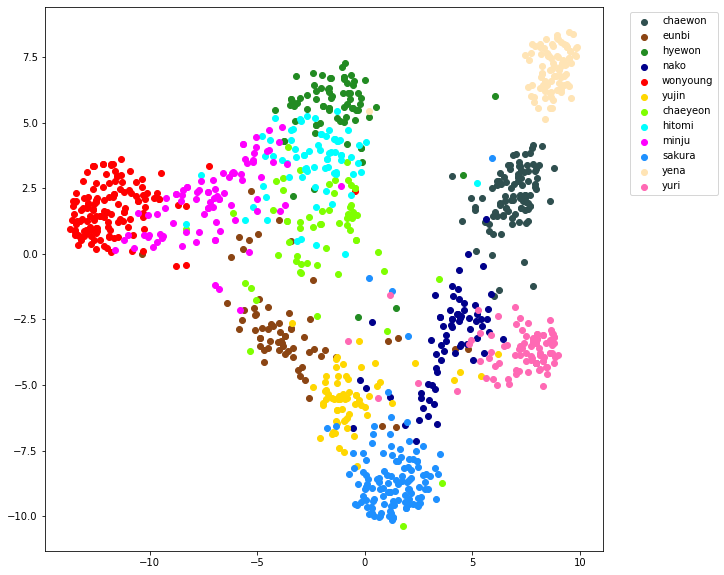
\includegraphics[trim=37 20 100 0, clip, width=\textwidth]{images/faceReco/nn2-and-triplet/tsne-1.png}     
    \end{subfigure}
    \hfill
    \begin{subfigure}{0.325\textwidth}
        \centering
        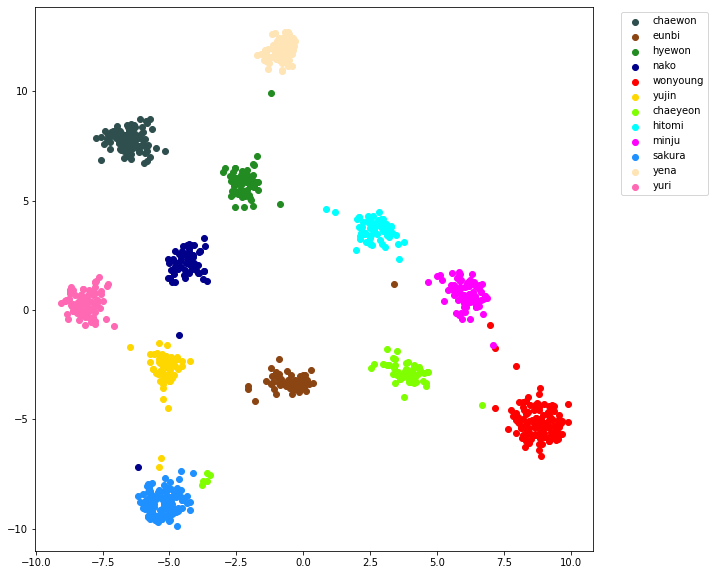
\includegraphics[trim=30 20 100 0, clip, width=\textwidth]{images/faceReco/nn2-and-triplet/tsne-2.png}     
    \end{subfigure}
    \hfill
    \begin{subfigure}{0.325\textwidth}
        \centering
        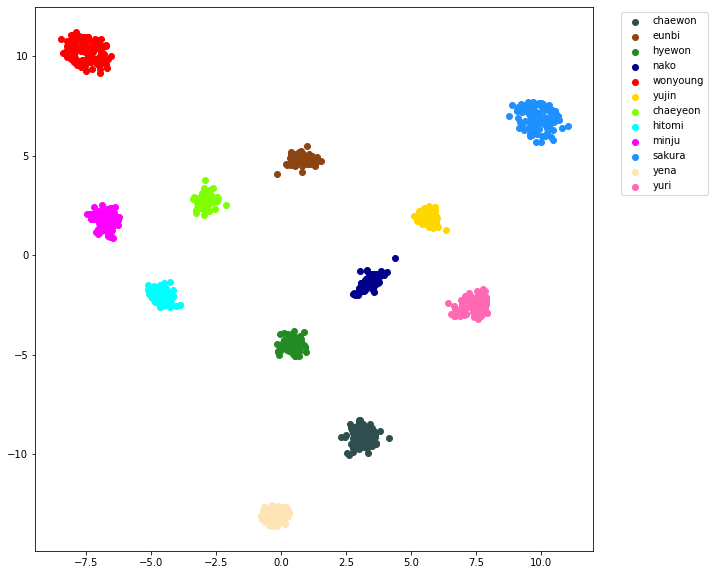
\includegraphics[trim=30 20 100 0, clip, width=\textwidth]{images/faceReco/nn2-and-triplet/tsne-3.png}     
    \end{subfigure}

    \caption{
        Sequence of t-SNE plots taken at various points during the training of NN2 with the triplet loss function technique.
        From left-to-right, the plots were taken after training on: 12800, 24320, 24480 samples.
    }
    \label{Figure:Face-Recognition:Results:nn2-and-triplet-tsne-sequence}
\end{figure}

\begin{figure}[htbp]
    \centering
    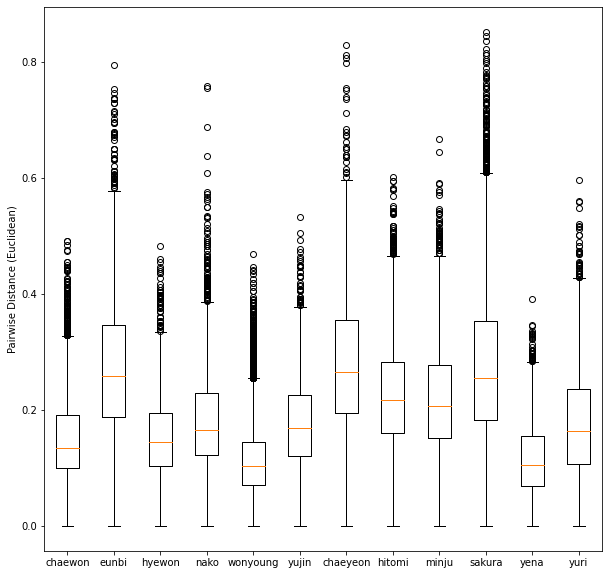
\includegraphics[width=0.7\textwidth]{images/faceReco/nn2-and-triplet/boxplot}
    \caption{Boxplot of pairwise distances for the training of NN2 with the triplet loss function technique}
    \label{Figure:Face-Recognition:Results:nn2-and-triplet-boxplot}
\end{figure}


\item \it{NN2 and Binary Classification Training}

The results for this experiment is similar to the previous one. 
The t-SNE plots in \Cref{Figure:Face-Recognition:Results:nn2-and-binary-tsne-sequence} show well-defined clusters and we can confirm with \Cref{Figure:Face-Recognition:Results:nn2-and-binary-boxplot} that the dispersion of image embeddings within clusters are quite low.
Once we examine \Cref{Table:Face-Recognition:Results:nn2-and-binary-medoid}, we see that the maximum intra-cluster distance of 0.12 is \it{very} low compared to the inter-cluster distance, which are all $>1$.
In fact, solely based on these tools, the best performance came from this experiment!

\begin{figure}[htbp]
    \centering
    \begin{subfigure}{0.325\textwidth}
        \centering
        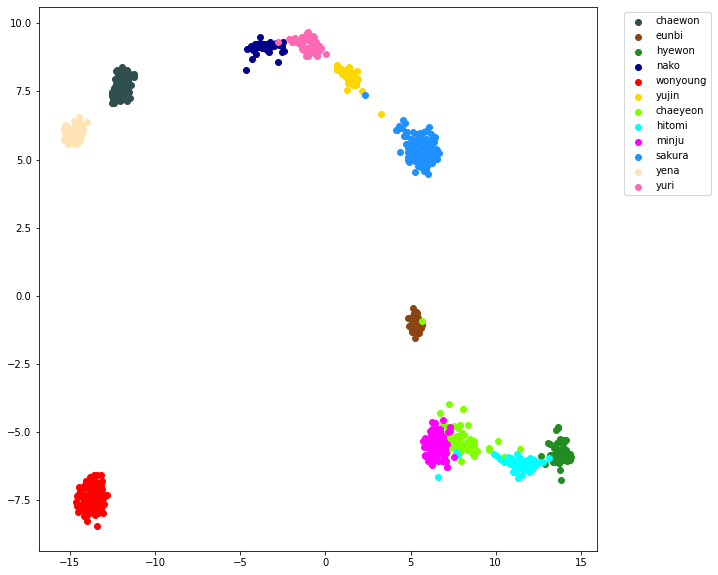
\includegraphics[trim=31 20 100 0, clip, width=\textwidth]{images/faceReco/nn2-and-binary/tsne-1.png}     
    \end{subfigure}
    \hfill
    \begin{subfigure}{0.325\textwidth}
        \centering
        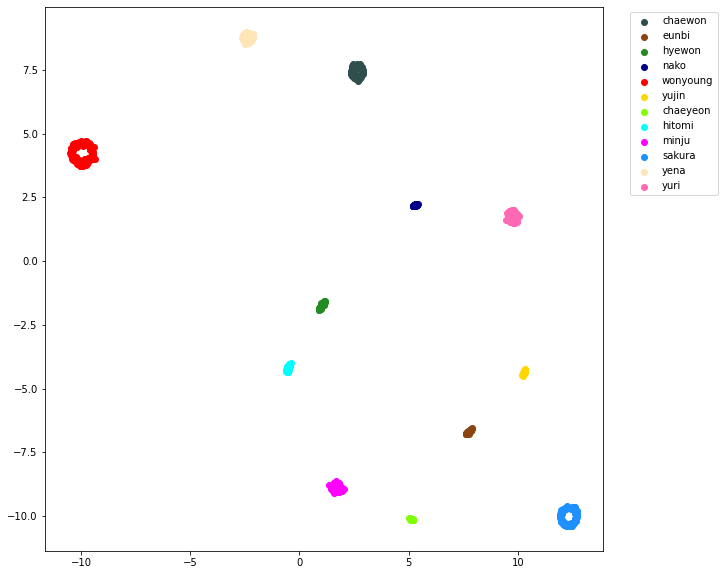
\includegraphics[trim=35 20 100 0, clip, width=\textwidth]{images/faceReco/nn2-and-binary/tsne-2.png}     
    \end{subfigure}
    \hfill
    \begin{subfigure}{0.325\textwidth}
        \centering
        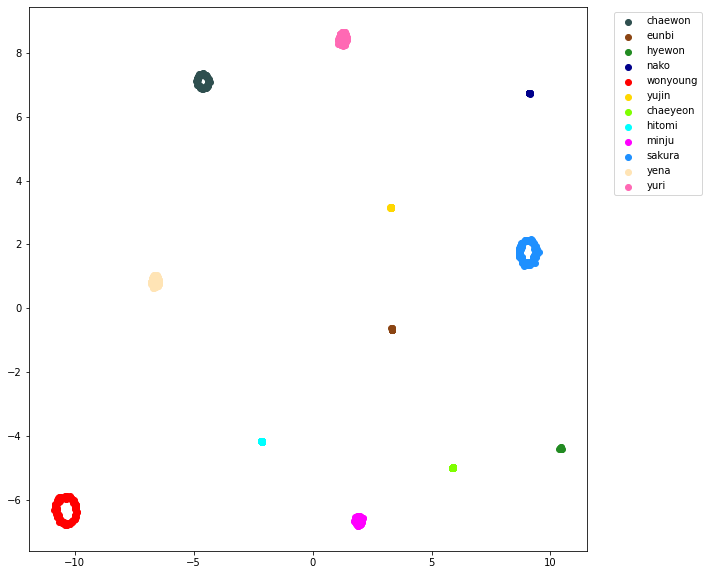
\includegraphics[trim=26 20 100 0, clip, width=\textwidth]{images/faceReco/nn2-and-binary/tsne-3.png}     
    \end{subfigure}

    \caption{
        Sequence of t-SNE plots taken at various points during the training of NN2 with the binary classification technique.
        From left-to-right, the plots were taken after training on: 80000, 160000, 304640 samples.
    }
    \label{Figure:Face-Recognition:Results:nn2-and-binary-tsne-sequence}
\end{figure}

\begin{figure}[htbp]
    \centering
    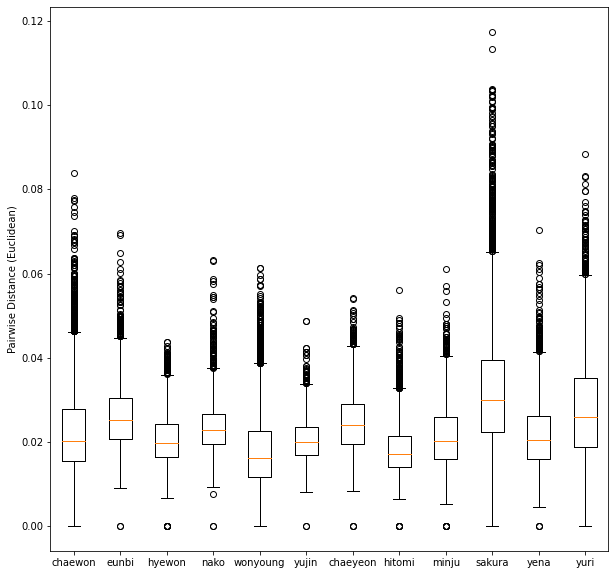
\includegraphics[width=0.7\textwidth]{images/faceReco/nn2-and-binary/boxplot}
    \caption{Boxplot of pairwise distances for the training of NN2 with the binary classification technique}
    \label{Figure:Face-Recognition:Results:nn2-and-binary-boxplot}
\end{figure}


\item \it{InceptionNetV3 and Triplet Loss}

Finally, we get to the last experiment, where we train the pre-built \it{Keras InceptionV3} with pre-loaded \it{imagenet} weights.
There is not much to say about this experiment since the architecture of InceptionV3 is similar to that of NN2.
As such, as one might expect, we get similar looking results as with the \it{NN2 and Triplet Loss} experiment.

\begin{figure}[htbp]
    \centering
    \begin{subfigure}{0.24\textwidth}
        \centering
        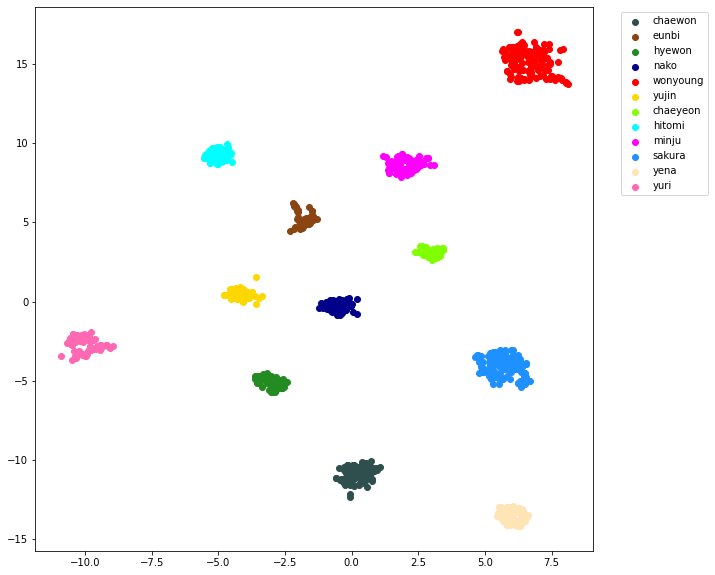
\includegraphics[trim=31 20 100 0, clip, width=\textwidth]{images/faceReco/inceptionv3-and-binary/tsne-1.png}     
    \end{subfigure}
    \hfill
    \begin{subfigure}{0.24\textwidth}
        \centering
        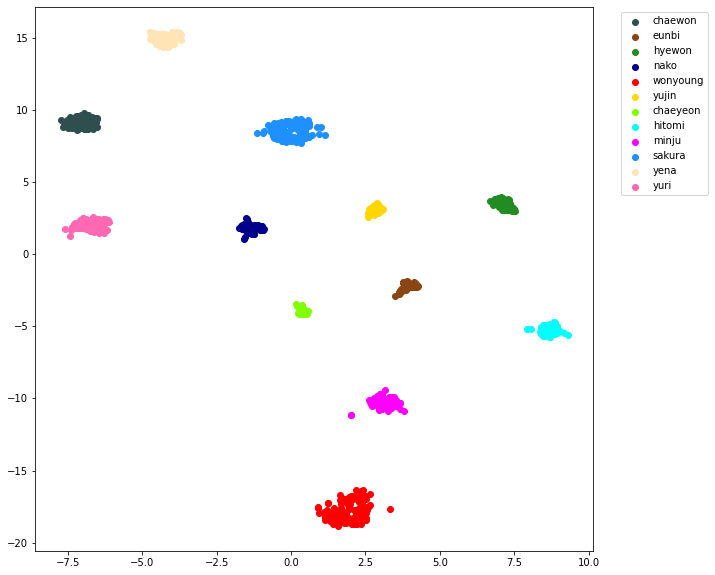
\includegraphics[trim=35 20 100 0, clip, width=\textwidth]{images/faceReco/inceptionv3-and-binary/tsne-2.png}     
    \end{subfigure}
    \hfill
    \begin{subfigure}{0.24\textwidth}
        \centering
        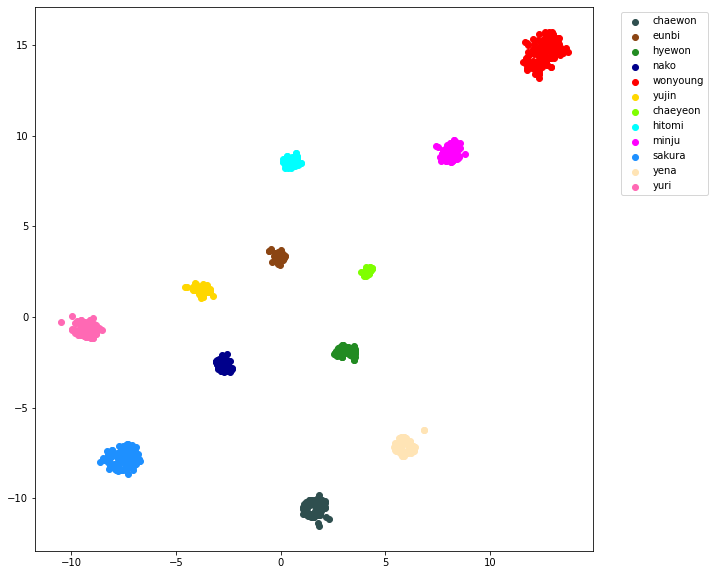
\includegraphics[trim=26 20 100 0, clip, width=\textwidth]{images/faceReco/inceptionv3-and-binary/tsne-3.png}     
    \end{subfigure}
    \hfill
    \begin{subfigure}{0.24\textwidth}
        \centering
        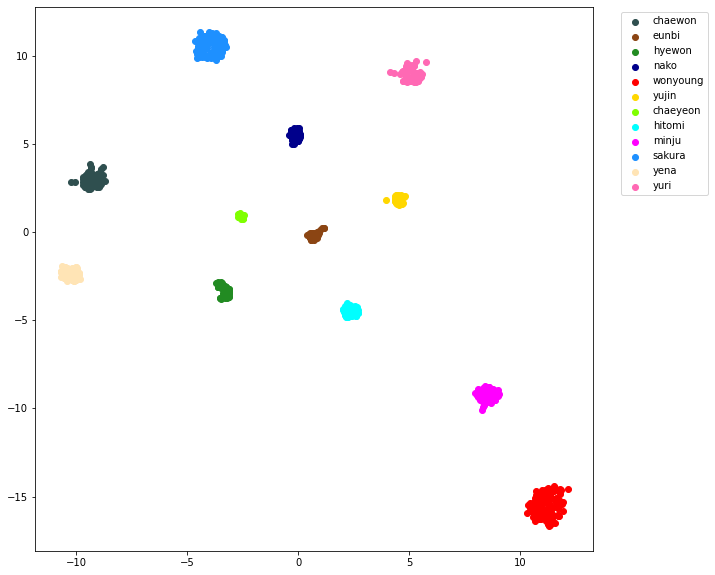
\includegraphics[trim=26 20 100 0, clip, width=\textwidth]{images/faceReco/inceptionv3-and-binary/tsne-4.png}     
    \end{subfigure}


    \caption{
        Sequence of t-SNE plots taken at various points during the training of InceptionV3 with the binary classification technique.
        From left-to-right, the plots were taken after training on: 80000, 160000, 240000, 320000 samples.
    }
    \label{Figure:Face-Recognition:Results:inceptionv3-and-binary-tsne-sequence}
\end{figure}

\begin{figure}[htbp]
    \centering
    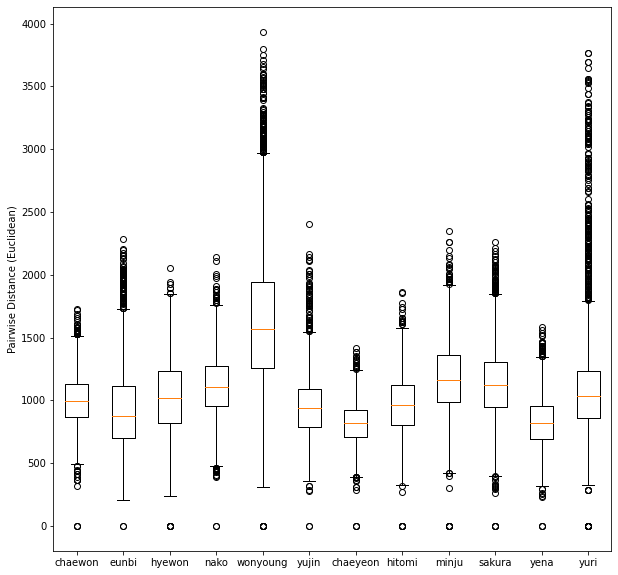
\includegraphics[width=0.7\textwidth]{images/faceReco/inceptionv3-and-binary/boxplot}
    \caption{Boxplot of pairwise distances for the training of InceptionV3 Net with the binary classification technique}
    \label{Figure:Face-Recognition:Results:inceptionv3-and-binary-boxplot}
\end{figure}


\end{enumerate}


